The task of recommender systems is to use users' data and their current and historical preferences with the goal of making predictions about users' possible future likes and interests \cite{Lu2012}.

In recommender systems, \gls{ml} models are used to predict the rating $r_{ui}$ of a user $u$ on an item $i$.
At inference time, the system recommends to each user $u$ the items $I$ having highest predicted rating $r_{ui}$.
It is therefore necessary to collect user feedback, so that we can have a ground truth for training and evaluating our models.
Explicit Feedback is a rating explicitly given by the user to express their satisfaction with an item.
Implicit Feedback assumes that user-item interactions are an indication of preferences.

The two main approaches in recommender systems are \gls{cbf} and \gls{cf}, often combined in hybrid methods \cite{Ko2022}.

\gls{cbf} is a method for recommending articles with attributes similar to those that users like and recommends them based on article information \cite{Vallet2006}.
According to \textcite{salter2006cinemascreen}, such filtering has a major drawback: it recommends only data on articles that are closely related to data on articles that a user has considered in the past. Because of this, the system struggles to recommend new articles. 

\gls{cf} relies on user-item interactions, such as ratings or clicks, to identify patterns and recommend items that were liked by similar users.
It is effective, but suffers from 3 problems such as: the sparsity problem, that occurs when there is not enough data available for recommendation \cite{Plexousakis2005}.
Another important problem is the cold start problem, which occurs when there is no evaluation data, that is, when a new user enters the system \cite{WEI201729}.
Finally, gray sheep is a problem in which there is only a small number of users with similar evaluation data to that of the individual user, and thus there are difficulties in providing recommendations \cite{Gras2016}.

Hybrid filtering systems integrate multiple recommendation techniques, such as \gls{cbf} and \gls{cf}, to address the shortcomings of each method and improve overall recommendation quality \cite{Ko2022}.
By combining these approaches, hybrid systems can utilize both item attributes and user behavior to create a more comprehensive understanding of preferences.
This combination enhances recommendation accuracy, increases diversity, and provides a more robust solution adaptable to various scenarios, making hybrid systems a superior choice for personalized recommendations.

\subsection*{Recommender Systems in Research Field}\label{sec:recommender-systems-in-research-field}
Most of the existing works of recommender systems in the literature regarding the field of research are based on suggesting research papers, or academic collaborators.
The following describes the work found during the literature review regarding these systems.

\textcite{refore} proposed the REFORE system, a hybrid recommender system specifically designed to assist researchers in managing information overload by providing high-quality and personalized recommendations of research papers.
The system integrates bibliometric measures, such as journal impact factors and author H-indexes, into its recommendation process, thereby emphasizing the quality of both the items (papers) and the users (researchers) involved.
REFORE employs a \gls{cbf} approach to match user preferences with paper content, using metadata such as keywords, abstracts, and citations.
It represents papers as vectors in a linguistic framework, assigning importance scores to keywords, which are then matched to user profiles.
The structure of the system is shown in Fig.~\ref{fig:refore}.
These profiles are built dynamically based on the researcher's past publications and manually input preferences.
Additionally, a \gls{cf} mechanism is implemented to leverage the feedback and preferences of similar users, identifying relevant items based on shared interests.
The system adopts a two-phase feedback process: users can evaluate recommendations as relevant or irrelevant and later provide qualitative assessments of the papers they read.
This feedback not only improves future recommendations but also helps refine the underlying quality measures for papers and authors.
A key innovation in REFORE is its re-ranking process, which combines \gls{cbf} and \gls{cf} outputs with quality scores derived from bibliometric data.
Papers are ranked not only by their relevance to the user but also by their scientific quality and novelty.
To handle the fuzziness inherent in user preferences and item quality, REFORE utilizes a fuzzy linguistic modeling approach, which ensures flexibility and granularity in assessing and aggregating preferences.
This linguistic framework allows for precise and interpretable measurements of similarities and quality across items and users.

\begin{figure}[htbp]
    \centering
 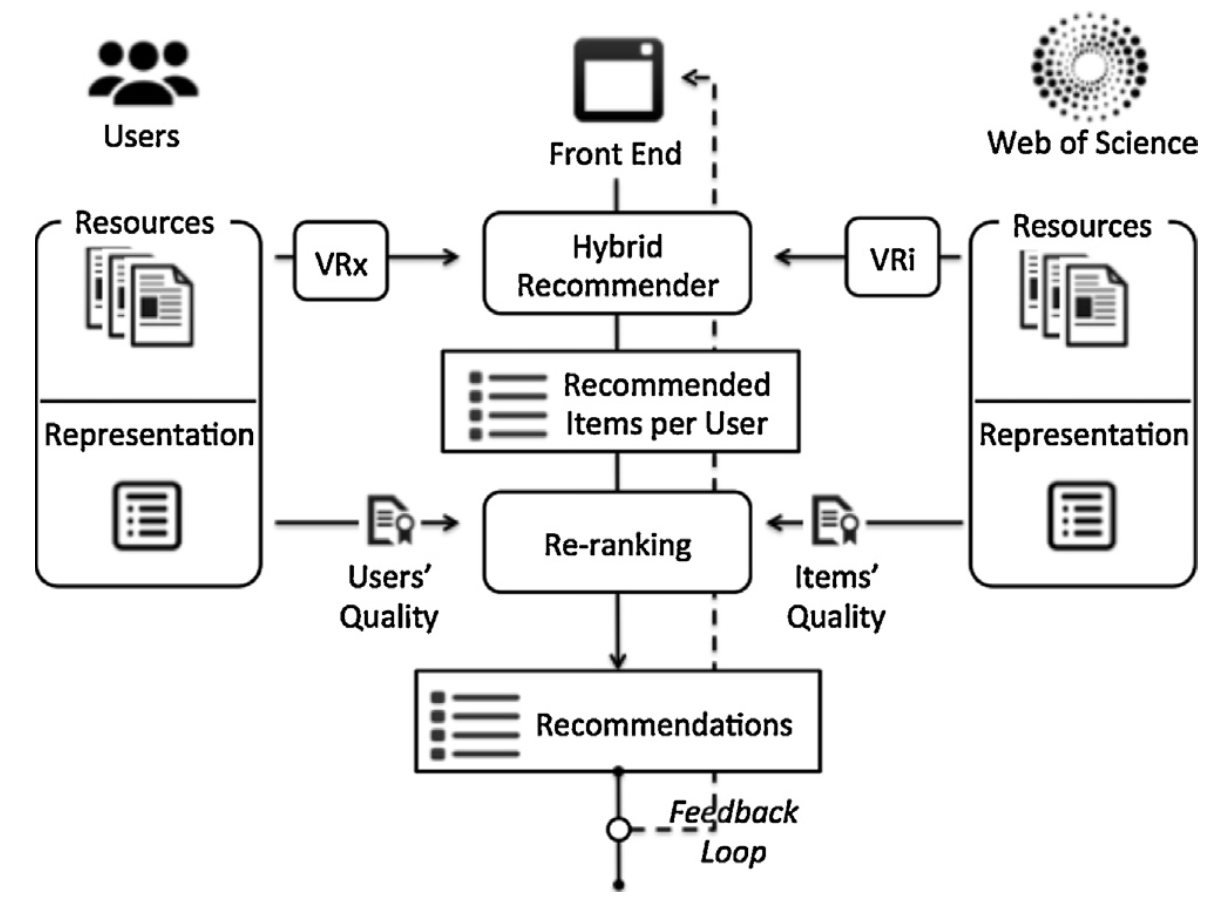
\includegraphics[width=0.6\textwidth]{figures/literature-review/refore.png}
     \rule{35em}{0.5pt}
    \caption{Structure of REFORE system (\textcite{refore})}
 \label{fig:refore}
\end{figure}

In terms of evaluation, the system was tested with a group of researchers from multiple institutions over a year-long period.
Researchers received monthly recommendations based on newly published papers from the Web of Science database, and their feedback was collected to measure the system's effectiveness.
The experimental results demonstrated the system's ability to deliver high-quality and personalized recommendations, outperforming traditional methods by incorporating bibliometric quality measures and user feedback into the hybrid recommendation strategy.

\textcite{Kanwal2024} proposed a research paper recommendation system, integrating citation networks and collaboration networks to provide high-quality and relevant suggestions to researchers.
This approach, named \gls{rrmf}, addresses challenges such as the cold-start problem, data sparsity, and semantic ambiguity.
The proposed methodology involves generating a multi-level citation network, where the focal paper of interest (PI) serves as the central node.
Citation relationships are explored up to six levels, leveraging both forward (citing) and backward (cited by) links.
To evaluate the relevance of papers within the network, bibliographic coupling and co-citation strengths are computed, quantifying the similarity of papers based on shared citations or references.
A candidate score is derived for each paper, which is used to filter irrelevant documents and focus on those most closely related to the paper of interest.
Additionally, centrality measures (such as betweenness, degree, closeness, and eigenvector centrality) are applied to rank papers based on their structural significance within the network.
Papers with high centrality scores are selected for further analysis.
The system extends beyond citation networks by incorporating collaboration networks of authors.
Authors are extracted from top-ranked papers, and their collaboration networks are analyzed using centrality and social measures to identify influential researchers.
These author-based insights contribute to refining paper recommendations, ensuring that suggested papers come from prominent authors within the field.
To evaluate the system, the AMiner dataset, comprising nearly 4.8 million papers and over 45 million citation relationships, was used.
The system's performance was benchmarked using metrics such as \gls{map}, \gls{mrr}, and \gls{ndcg}.
Experimental results demonstrated that the \gls{rrmf} outperformed traditional systems, such as Google Scholar and previous citation-based methods, by achieving higher precision and recall.
The incorporation of multi-level citation analysis and author collaboration measures significantly improved the quality and relevance of recommendations.

\textcite{Murali2019} proposed a research paper recommender system using a user-based \gls{cf} approach.
The goal of the system is to recommend research papers tailored to a user's interests by analyzing their preferences and similarities with other users.
The authors addressed the challenge of information overload faced by researchers due to the rapid growth in the number of research publications.
The system operates by collecting a dataset of user-paper interactions, which includes attributes such as user IDs, paper IDs, and ratings assigned by users to the papers. Based on this data, the system calculates the similarity between users using the cosine similarity measure. This approach evaluates the resemblance between user profiles by treating their preferences as vectors and computing the cosine of the angle between them.
Users with similar interests are identified, and recommendations are generated by predicting ratings for papers based on the ratings given by these similar users.
The block diagram of the system architecture is shown in Fig.~\ref{fig:murali}.
To improve the quality of recommendations, the system utilizes a prediction rating mechanism, which assigns a predicted score to papers based on the \gls{cf} model.
Papers with higher predicted ratings are recommended to the user, ensuring that suggestions align with their preferences.
The authors also implemented a ``user-link formation'' step to construct the \gls{cf} model, leveraging the collective behavior of similar users to refine recommendations further.

\begin{figure}[htbp]
    \centering
 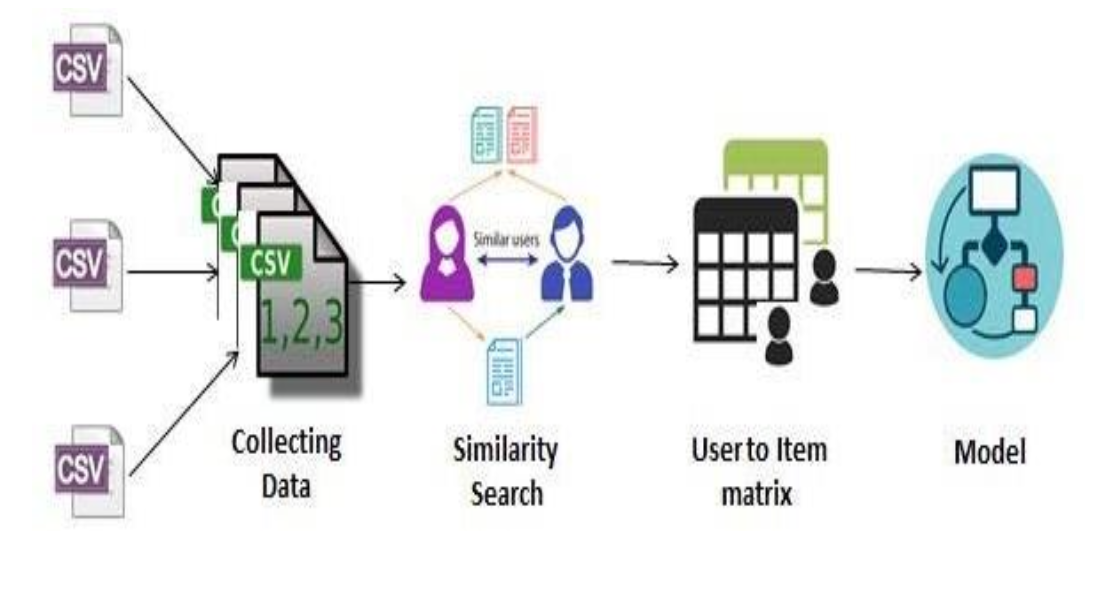
\includegraphics[width=0.65\textwidth]{figures/literature-review/murali.png}
     \rule{35em}{0.5pt}
    \caption{Block diagram of the system architecture (\textcite{Murali2019})}
 \label{fig:murali}
\end{figure}

For evaluation, the system was tested on a dataset comprising 135 users and their interactions with research papers.
Performance was measured using metrics like \gls{mae} and \gls{rmse} to assess the accuracy of predicted ratings against actual ratings.
The results showed that the user-based \gls{cf} model performed well, producing high-quality recommendations with minimal deviation in predicted ratings.
The authors acknowledge limitations in their work, such as the reliance on a synthetic dataset for testing due to the unavailability of real-world datasets with pre-existing paper ratings.
They suggest that the system's effectiveness could be further enhanced if real datasets from platforms like research paper repositories were used.

In their work, \textcite{Sharma2023} present a detailed exploration of research paper recommender systems, addressing their evolution, methodologies, and associated challenges.
It categorizes existing approaches into key methodologies, including \gls{cbf}, \gls{cf}, link-based algorithms, co-occurrence techniques, and hybrid approaches.
Each method is analyzed based on its underlying knowledge sources, such as textual attributes of research papers, author profiles, citation patterns, and user-generated tags, which are leveraged to model user preferences and generate personalized recommendations.
Based on their studies, the authors divide recommender systems into three essential components: the first requirement for performing any task is domain-specific knowledge and its application to the task at hand.
This is called principle or basic knowledge and operational theory.
Principle knowledge includes all available information about an item that is used to perform the recommendation task and serves as key attributes of the system to generate recommendations.
Operational theory, on the other hand, is concerned with the ``how'' aspect, i.e., how the information provided is applied to achieve the intended goals.
The second component is the recommendation approach, which outlines a step-by-step methodology for solving the problem, detailing implementation techniques and their practical implementation.
Finally, the third component, probably the most critical, is user modeling.
The general architecture of a research paper recommendation system is shown in Fig.~\ref{fig:general-architecture-rprs}.

\begin{figure}[htbp]
    \centering
 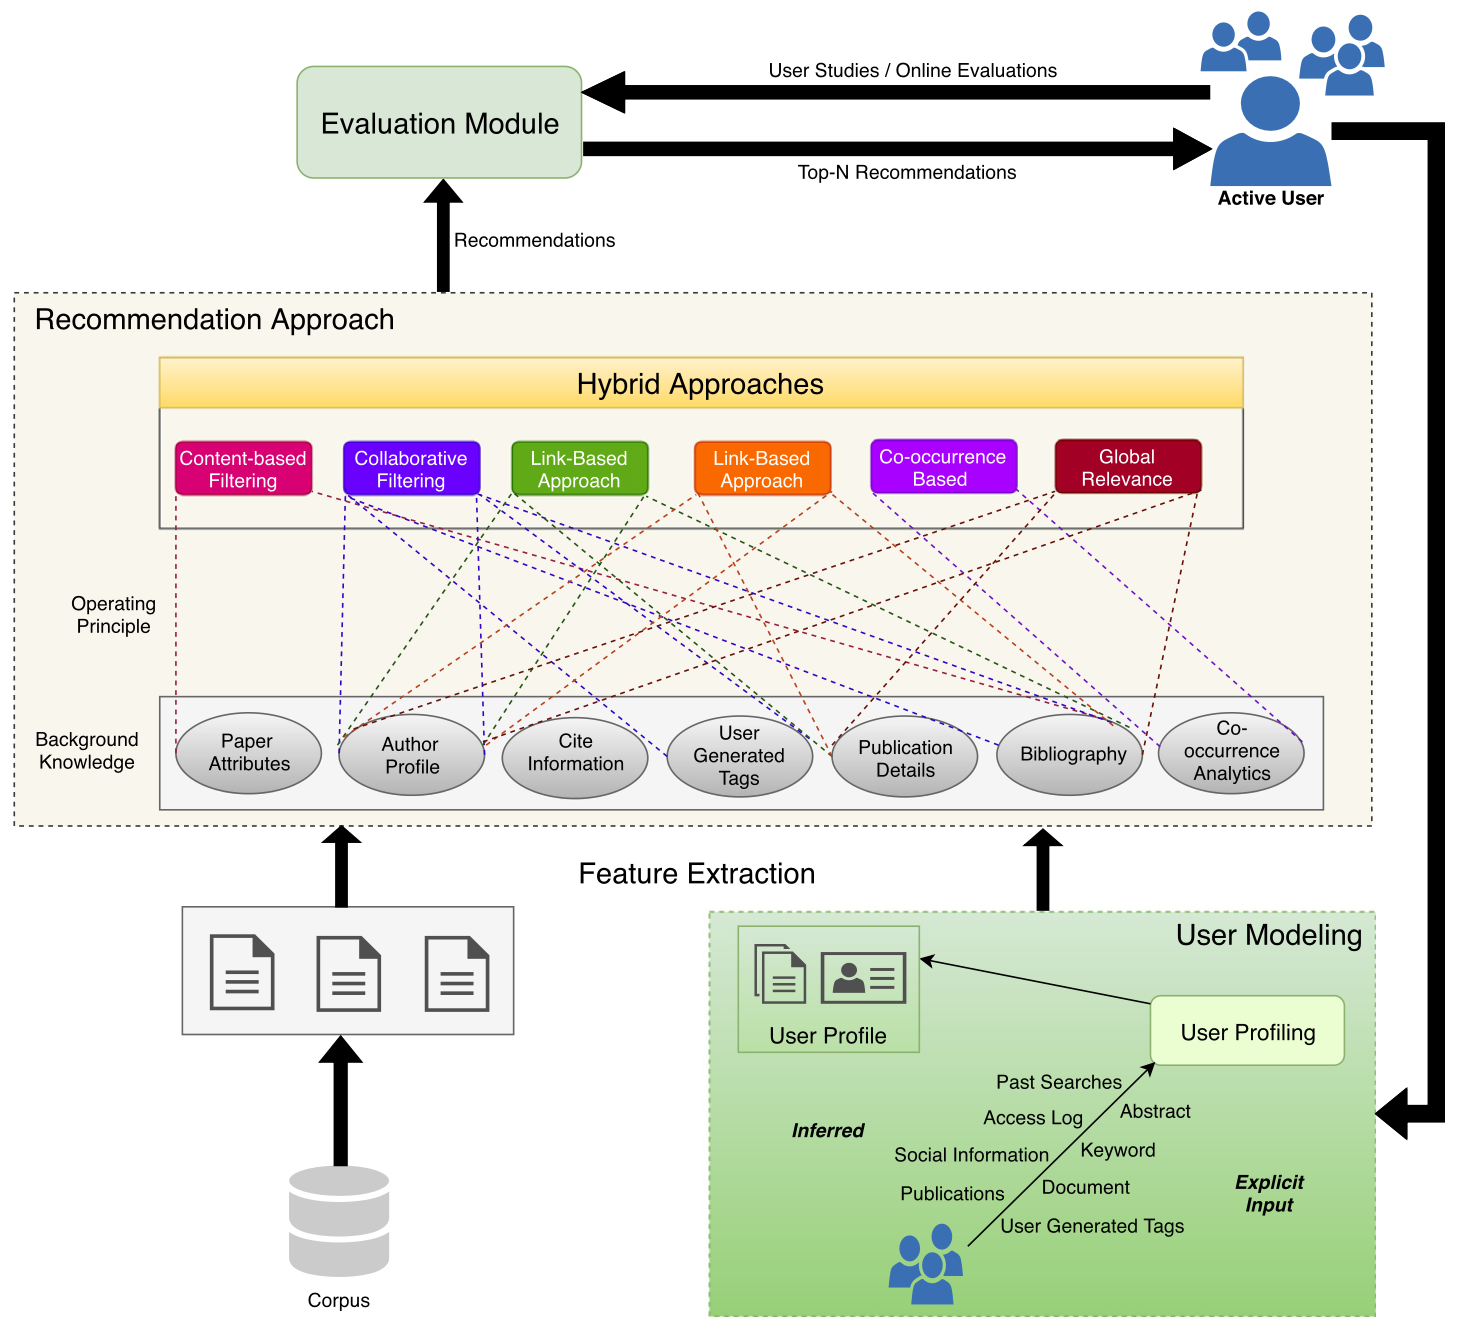
\includegraphics[width=0.7\textwidth]{figures/literature-review/general-architecture-rprs.png}
     \rule{35em}{0.5pt}
    \caption{General architecture of Research Paper Recommendation System (\textcite{Sharma2023})}
 \label{fig:general-architecture-rprs}
\end{figure}

The authors highlight the dominance of \gls{cbf} techniques, which rely on textual similarity between papers and user profiles, and discuss how \gls{cf} leverages peer preferences to improve recommendations.
Hybrid methods, which integrate multiple approaches, are presented as a solution to address the limitations of individual techniques, such as over-specialization in \gls{cbf} and data sparsity in \gls{cf}.
The study also identifies critical challenges, including the lack of standard datasets for benchmarking, insufficient evaluation metrics for dimensions like novelty and serendipity, and the difficulty of scaling algorithms to handle real-world, large-scale datasets.
Furthermore, the paper underscores the need for more sophisticated evaluation frameworks and advanced computational models, such as \gls{dl}, to improve the efficacy and scalability of research paper recommender systems.

\textcite{Jagadishwari2023} proposed a methodology for recommending academic collaborators using a combination of citation analysis and academic influence metrics.
Their work highlights the importance of identifying suitable collaborators to enhance research productivity and addresses the challenges posed by the vast volume of academic data.
The system utilizes the DBLP dataset \cite{Ley2002}, focusing on core computer science publications from 2017 to 2019, and incorporates citation count and influential citation metrics to assess academic influence.
The methodology involves preprocessing the dataset to eliminate irrelevant data, computing an Academic Level Index (ALI) using three different formulae, and then calculating a Research Score (R score) based on ALI and domain-specific publication metrics.
The R score serves as the basis for ranking scholars and identifying potential collaborators.
Three variations of the R score computation are tested, and the study concludes that the third formula (R3 Score) yields the most compatible recommendations by minimizing differences between the scores of the target scholar and recommended collaborators.
The system's results are visualized using graphs and compared across the three scoring methods, demonstrating that R3 Score provides the most precise matches.
The authors suggest future research could include additional factors like geographic location and funding status, as well as expanding the dataset to other academic disciplines.

\textcite{Zhang2023} provide a comprehensive review of scholarly recommendation systems, highlighting their evolution, methodologies, applications, and challenges.
These systems play a crucial role in academia, assisting researchers in identifying relevant literature, potential collaborators, conferences, journals, datasets, and grant opportunities.
The study identifies \gls{cbf} as the most widely used technique, particularly for literature recommendations, whereas \gls{cf} is more prevalent in conference and collaborator recommenders.
Hybrid approaches, which combine \gls{cbf} and \gls{cf}, are also discussed as a promising direction for improving recommendation accuracy and diversity.
The paper evaluates 225 publications across various SRS domains, showing that literature and collaborator recommendation systems dominate the field, while systems for datasets and grants are underexplored.
It notes the limited adoption of deep learning methods in scholarly recommendation systems and emphasizes the need for better integration of user feedback mechanisms to enhance system personalization and effectiveness.
Furthermore, the study highlights the challenges of scalability, data sparsity, and the cold start problem in existing systems.
Evaluation methods, including online and offline metrics, are examined, with offline evaluations being the most common.
In its conclusion, this work stresses the importance of developing unified frameworks that integrate diverse methodologies and leverage advances in \gls{ai} to address current limitations.
It also calls for more research into underrepresented areas like dataset and grant recommendation systems, advocating for user-centric designs that prioritize usability and practical application.

\textcite{Du2022} propose a novel model called ACR-ANE to enhance the recommendation of academic collaborators by integrating network topology and multi-type scholar attributes.
The study addresses the limitations of existing approaches, which often consider only local network structures or singular attribute types, and introduces non-local neighbors to capture stronger academic relationships.
Non-local neighbors are determined through biased random walks and frequency filtering, allowing the model to identify significant connections beyond immediate collaborators.
The methodology incorporates six scholarly attributes-academic age, research interests, publication count, average citations, number of collaborators, and H-index, into a scholar attribute matrix.
These attributes, combined with network structure, are encoded using a deep auto-encoder to generate low-dimensional embeddings that preserve both local and global academic network characteristics.
The model establishes a new multi-type relational network by integrating non-local neighbors and attribute-based proximity, which enriches the representation of academic relationships.
The framework of ACR-ANE is shown in Fig.~\ref{fig:acr-ane}.

\begin{figure}[htbp]
    \centering
 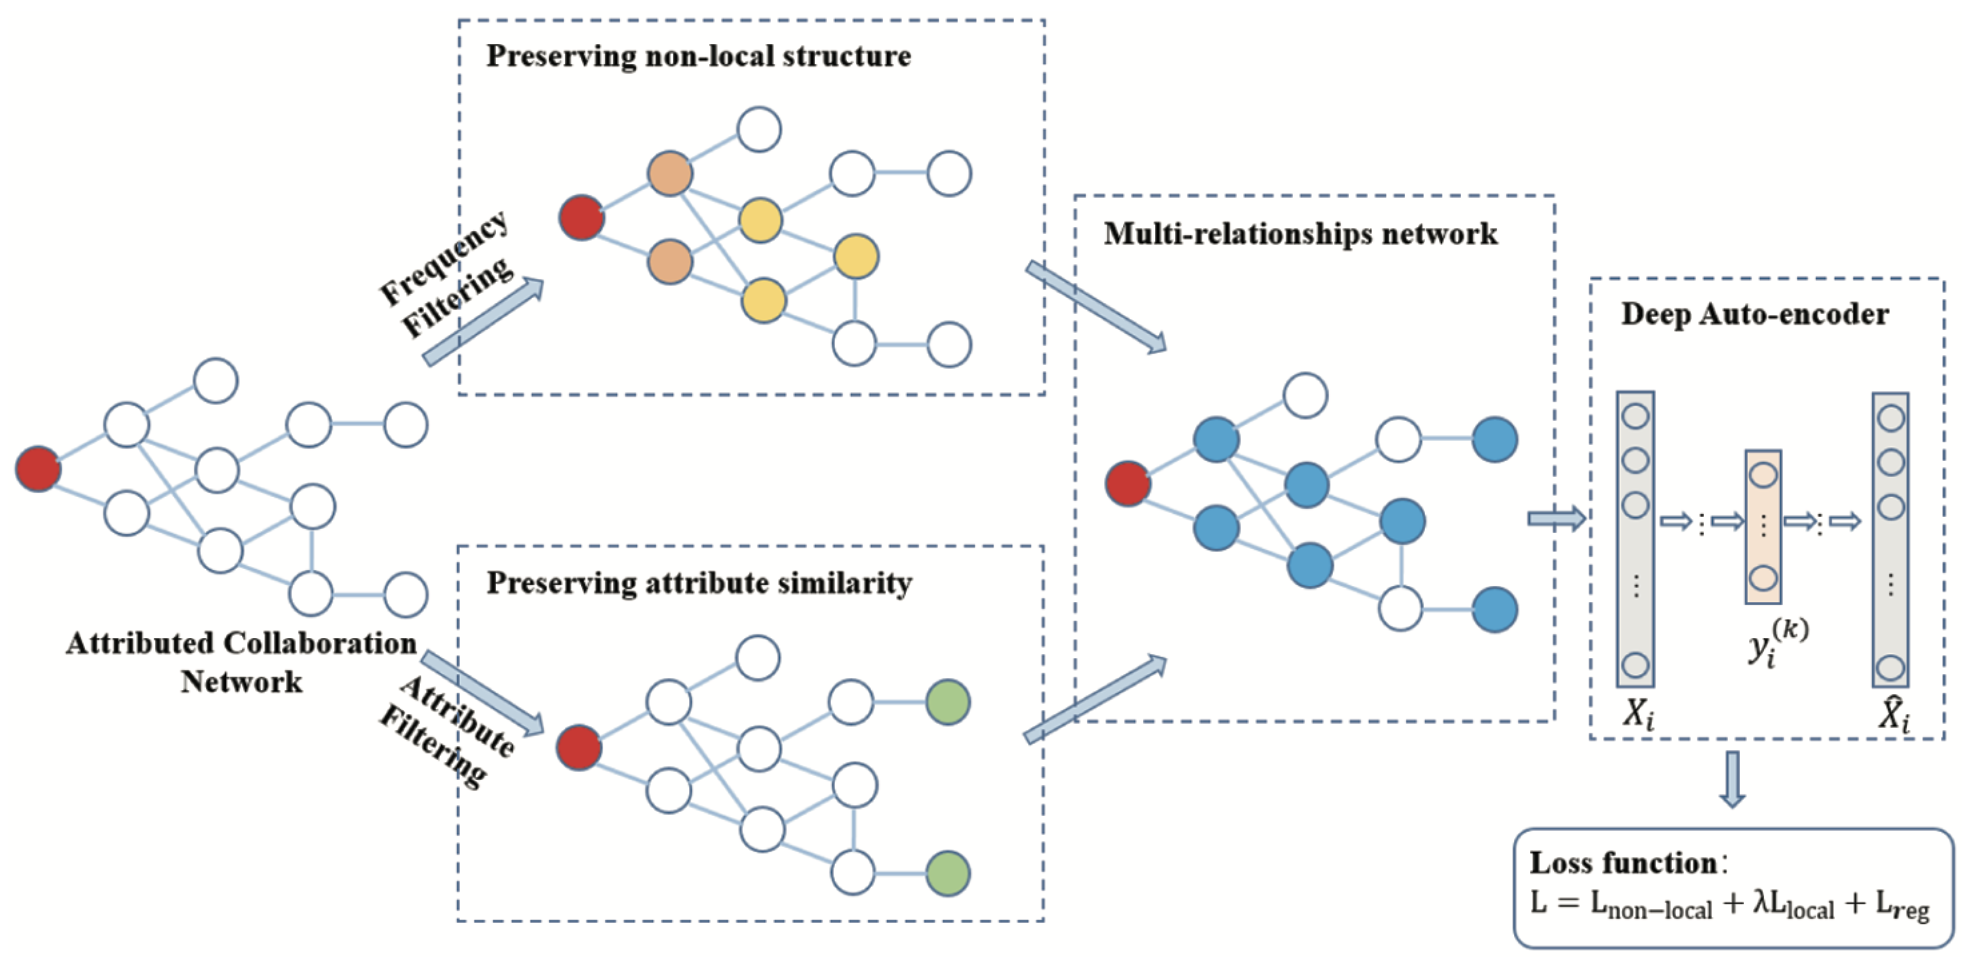
\includegraphics[width=0.8\textwidth]{figures/literature-review/academic-collaborator-recommendation-framework.png}
     \rule{35em}{0.5pt}
    \caption{The framework of ACR-ANE model. (\textcite{Du2022})}
 \label{fig:acr-ane}
\end{figure}

Extensive experiments conducted on two real-world datasets, Aminer and APS, demonstrate the superior performance of ACR-ANE in comparison to baseline models such as DeepWalk, TADW, SDNE, and ACNE.
The results highlight the effectiveness of combining network structure and scholar attributes for collaborator recommendation.
However, the study acknowledges its limitation in handling dynamic networks and suggests future work on incorporating temporal factors to reflect evolving academic collaborations.

\textcite{Zhu2022} explore the application of \glspl{gnn} to recommend research collaborators in the academic domain.
The study focuses on leveraging dynamic and temporal aspects of research networks, addressing the challenge of identifying suitable collaborators in a rapidly evolving academic landscape.
The authors utilize data from the MEDLINE database and implement two \gls{gnn}-based models, GraphSAGE and \gls{tgn}, to capture both static and temporal dependencies among researchers.
GraphSAGE employs an inductive approach that generates embeddings for unseen nodes by aggregating neighbor features, making it suitable for large and dynamic graphs.
\gls{tgn} extends this by incorporating temporal elements, using a message-passing mechanism to update node embeddings based on time-stamped interactions.
These models are compared against baseline methods, including the transductive LightGCN and a \gls{gbc}.
The study is divided into two experimental scenarios: automatic evaluations using \gls{auc} and average precision metrics, and external evaluations based on user ratings collected via a web-based application.
Results indicate that \gls{tgn} outperforms other methods in handling temporal dynamics and inductive tasks, particularly when using publication titles as node features.
While GraphSAGE exhibits strong performance for static embeddings, \gls{tgn} demonstrates superior capability in predicting future collaborations by integrating time-sensitive relationships.
The authors acknowledge limitations such as the small sample size in external evaluations and the reliance on static node features for some tests.
They propose future enhancements, including the integration of distribution-based representations for nodes to better manage uncertainty and improve predictive modeling.

\subsection*{Retrieval-Augmented Recommender Systems}\label{sec:retrieval-augmented-recommender-systems-in-research-field}

As described in Sec.~\ref{sec:retrieval-augmented-generation} and according to \textcite{Deldjoo2024}, \gls{rag} leverages the integration of retrieval systems and generative models to produce highly relevant and context-aware recommendations.
This approach stores knowledge externally, allowing dynamic updates and reducing the risk of hallucinations by grounding outputs in retrieved data.
By minimizing the need for extensive model parameters, \gls{rag} improves efficiency and makes complex tasks, such as generating personalized explanations, more feasible.
However, its effectiveness is strictly linked to the quality and relevance of the retrieved information, making it reliant on robust retrieval systems and well-curated external knowledge bases.
Additionally, the integration of retrieval and generation components introduces complexity and potential computational overhead, especially in real-time applications.
Despite these challenges, \gls{rag} offers a powerful framework for enhancing the accuracy and adaptability of modern recommender systems.

For example, \textcite{Banerjee2024} propose an approach to improve tourism recommender systems by integrating sustainability considerations into the recommendation process.
The authors leverage \gls{rag} to enhance \glspl{llm} for generating recommendations, focusing on sustainable city trips in Europe.
Their main innovation is the incorporation of a sustainability metric during the \gls{rag} pipeline's prompt augmentation phase, called Sustainability Augmented Reranking (SAR).
Fig.~\ref{fig:sar-enhanced-recommendation} illustrates the SAR-enhanced recommendation process, which adjusts the traditional \gls{rag} pipeline by including a sustainability metric based on city popularity and seasonal demand.

\begin{figure}[htbp]
    \centering
    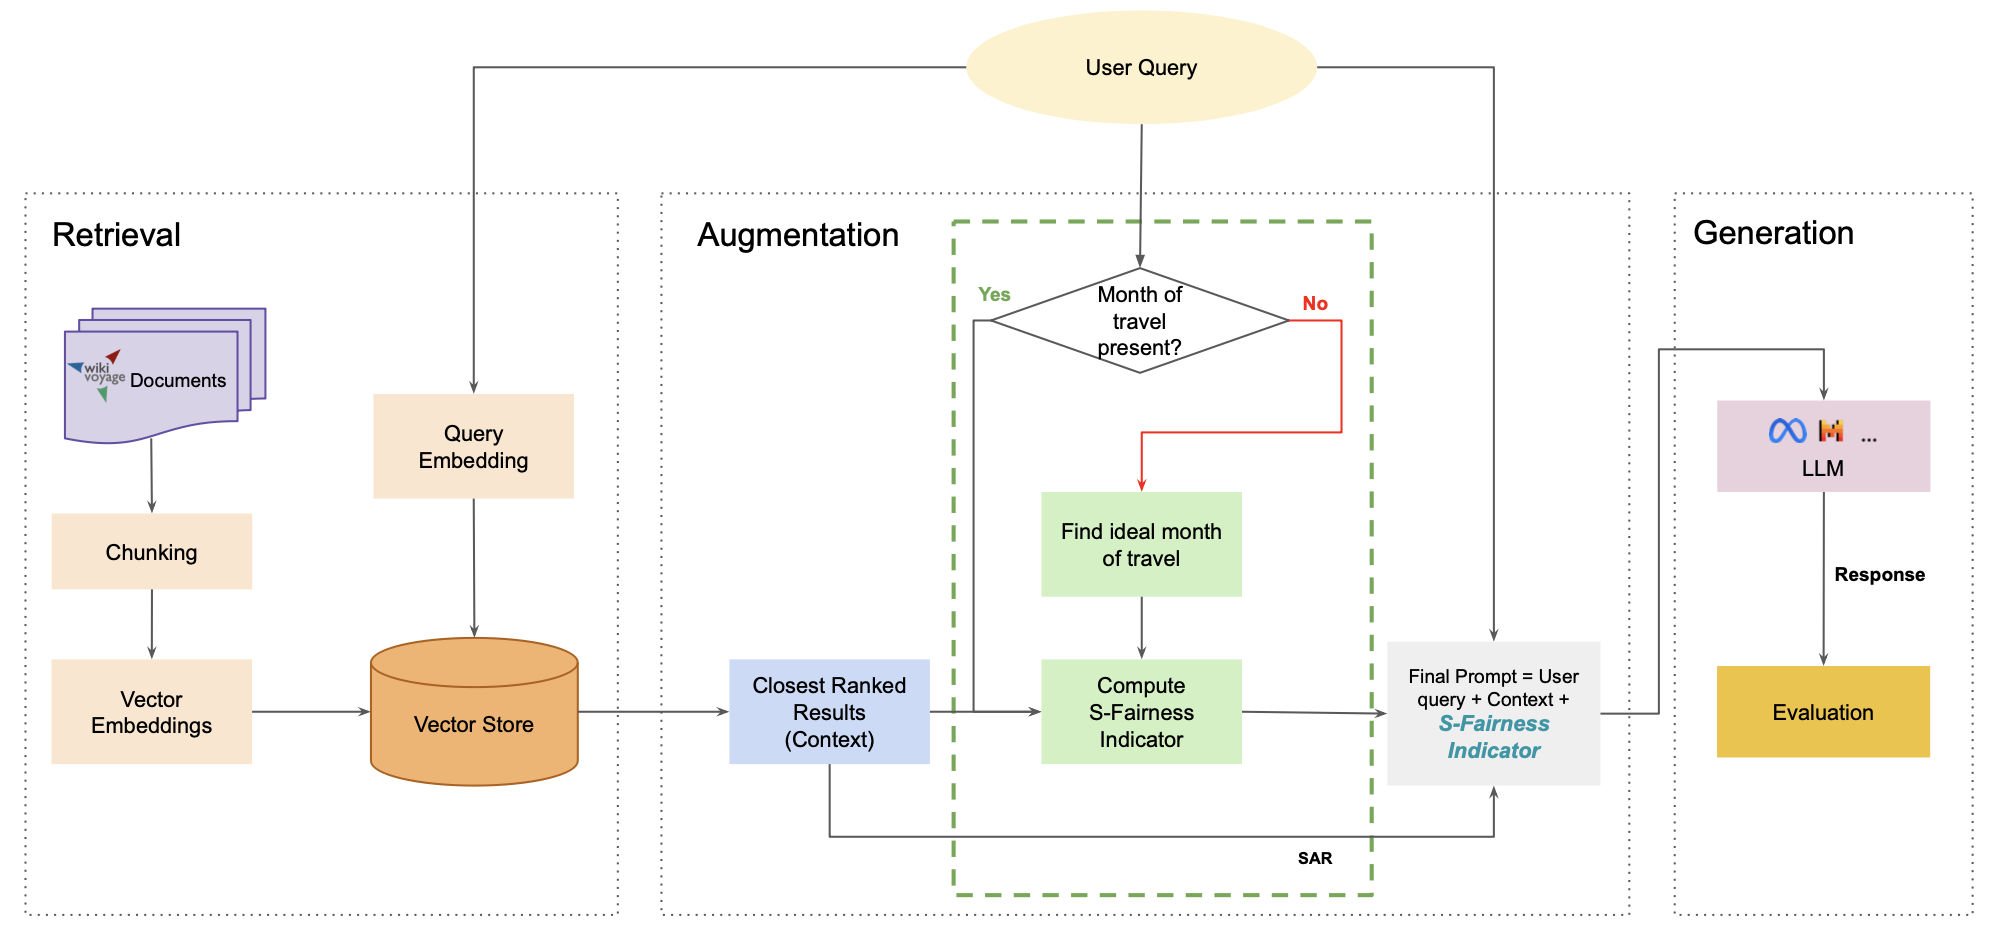
\includegraphics[width=0.8\textwidth]{figures/literature-review/rag-tourism.png}
    \rule{35em}{0.5pt}
    \caption{SAR-enhanced recommendation process (\textcite{Banerjee2024})}
 \label{fig:sar-enhanced-recommendation}
\end{figure}

The SAR enhancement adjusts the traditional \gls{rag} process by including a sustainability metric based on city popularity and seasonal demand.
This metric helps the system prioritize recommendations that align with sustainability principles, such as promoting destinations with lower tourism pressure during certain months.
By leveraging data from sources like Wikivoyage\footnote{\url{https://www.wikivoyage.org}} and Tripadvisor\footnote{\url{https://www.tripadvisor.com}}, the system calculates popularity and seasonality indices to inform the SAR metric, ensuring that recommendations balance user preferences with environmental and societal considerations.
Using open-source \glspl{llm}, such as Llama-3.1-Instruct-8B and Mistral-Instruct-7B, the study demonstrates that SAR-enhanced recommendations perform equal to or better than baseline models (without SAR) in terms of quality and sustainability.
The approach reduces common issues in \gls{llm}-based TRS, like hallucinations, and supports a multi-stakeholder perspective by addressing the needs of users, local communities, and environmental sustainability.

Another example is \gls{ramo}, a system designed to enhance Massive Open Online Courses (MOOCs) recommendations by addressing the ``cold start'' problem common in recommender systems \cite{Rao2024}.
Traditional course recommendation systems often struggle with new users due to the absence of historical data.
\gls{ramo} tackles this limitation by leveraging a \gls{rag} pipeline integrated with \gls{llm}.
In \gls{ramo}, the \gls{rag} framework combines two key components: a retriever and a generator.
The retriever accesses a pre-built knowledge base of course data, such as Coursera's publicly available dataset, and retrieves relevant information based on user queries.
The retrieved content is used to augment the prompts provided to the generator, ensuring responses are contextually relevant and precise.
This setup enables \gls{ramo} to generate personalized course recommendations even when little or no user-specific information is available, thereby overcoming the cold start issue.
The \gls{ramo} system workflow is shown in Fig.~\ref{fig:ramo-system-workflow}.

\begin{figure}[htbp]
    \centering
    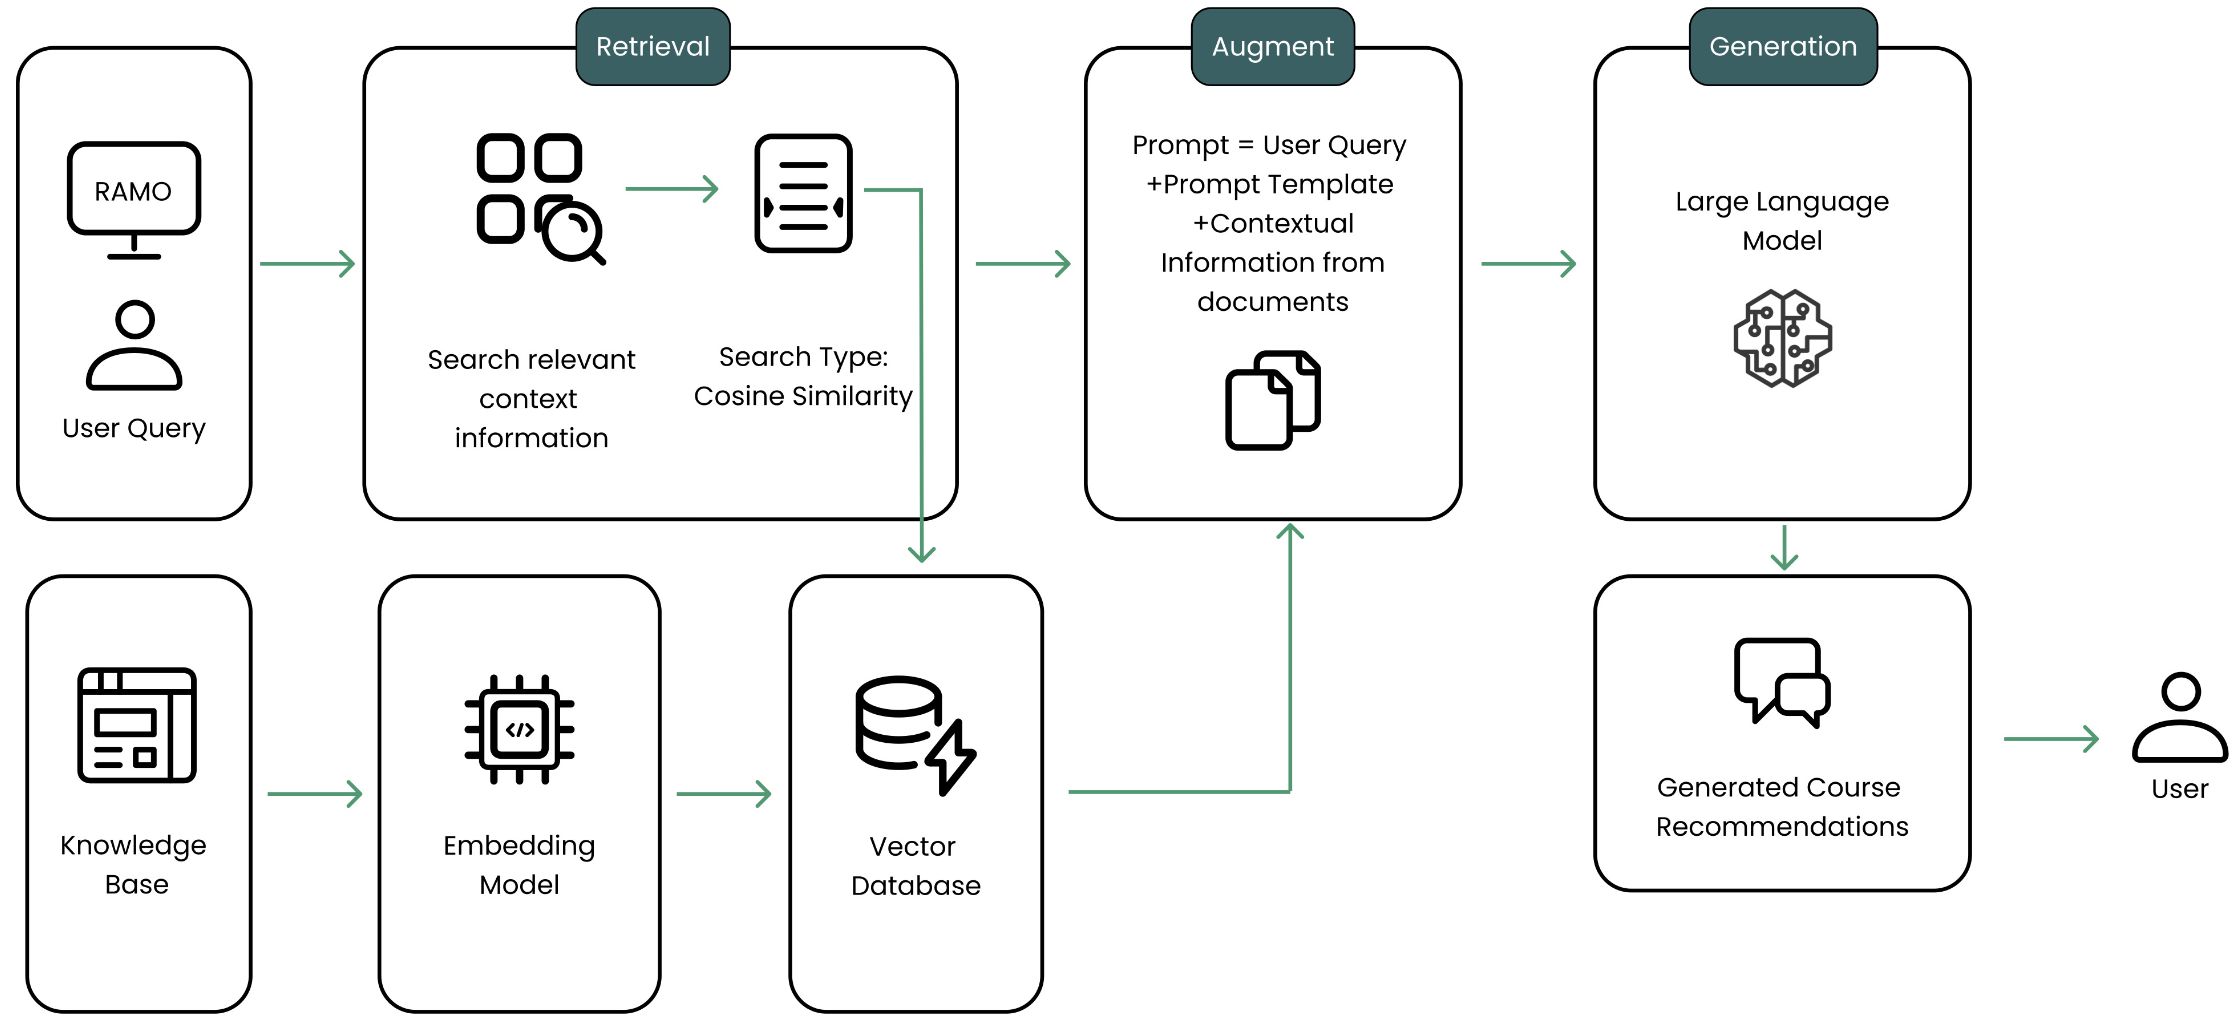
\includegraphics[width=0.8\textwidth]{figures/literature-review/ramo.png}
    \rule{35em}{0.5pt}
    \caption{The \gls{ramo} System workflow (\textcite{Rao2024})}
 \label{fig:ramo-system-workflow}
\end{figure}

The system utilizes advanced text embedding techniques to store and retrieve course data efficiently, employing models like OpenAI's text-embedding-ada-002 for embedding generation.
The final recommendations are produced by GPT-3.5 Turbo, selected for its cost-efficiency and performance, allowing dynamic, conversational interaction with users.
The paper evaluates \gls{ramo} by comparing its performance to traditional systems and standard \gls{llm}-based recommenders without \gls{rag}.
Results show that the \gls{rag}-enhanced system delivers more personalized and flexible recommendations, particularly in scenarios requiring personalized suggestions or dealing with general queries from new users.
The integration of \gls{rag} also ensures that the recommendations align closely with user needs by dynamically retrieving and incorporating domain-specific knowledge.

\textcite{DiPalma2023} explore the integration of \glspl{llm} into recommender systems to address challenges like cold-start problems, data sparsity, and adaptability to unseen data.
While traditional methods such as \gls{cf}, matrix factorization, and \gls{cbf} are effective in structured domains, they struggle in dynamic environments.
In contrast, \glspl{llm} leverage vast pre-trained knowledge, enabling them to generate meaningful recommendations even in novel scenarios.
To combine these strengths, the paper proposes a Retrieval-Augmented Recommender System that integrates retrieval-based and generative models to enhance accuracy and explainability.
This framework allows recommender systems to retrieve relevant external knowledge while using \glspl{llm} for improved reasoning and contextual adaptation.
The study examines \glspl{llm} in two roles: at the higher level, powering conversational \gls{ai} for personalized recommendations, and at the lower level, refining recommendation strategies through knowledge retrieval and generation.
Evaluating GPT-3.5 on MovieLens100K and Facebook Books datasets, the study compares its performance with state-of-the-art baselines using accuracy metrics such as nDCG, HR, and MAP.
GPT-3.5 performs competitively, particularly excelling in book recommendations due to its extensive pretraining on book-related data.
In movie recommendations, its performance is slightly lower than top models, highlighting the need for fine-tuning or retrieval augmentation.
Despite its potential, several challenges arise in integrating \glspl{llm} into recommender systems.
The cold-start problem persists, as effectiveness varies by dataset and domain.
Hallucination remains an issue, with models generating inaccurate or non-existent recommendations.
Popularity bias limits diversity, and the lack of real-time updates prevents awareness of newly introduced items.
Additionally, the black-box nature of \glspl{llm} raises concerns about explainability compared to traditional, more interpretable recommender systems.

\textcite{Wu2024} addresses the challenge of long-tail recommendation, where traditional \gls{cf}-based recommender systems struggle due to data sparsity and imbalance.
While \glspl{llm} have demonstrated strong reasoning capabilities, they typically rely on item semantics and fail to capture collaborative user-item interaction patterns, leading to misaligned recommendations.
To overcome this limitation, the authors introduce CoRAL, a collaborative retrieval-augmented \gls{llm} framework that integrates collaborative evidence into \gls{llm} prompts, ensuring alignment with real-world user-item interactions.
CoRAL enhances recommendation performance by retrieving minimal-sufficient collaborative information through a reinforcement learning-based retrieval policy, optimizing the inclusion of relevant interactions while minimizing unnecessary data that could distract the \gls{llm}.
The framework formulates long-tail recommendation as a sequential decision-making problem, where the retrieval policy dynamically selects user-item interactions to support the \gls{llm}'s reasoning process.
Experimental evaluations on Amazon product datasets demonstrate that CoRAL significantly outperforms both traditional \gls{cf} methods and standard \gls{llm}-based recommendation approaches, achieving superior accuracy in predicting user preferences.
The study highlights the importance of integrating collaborative knowledge with \glspl{llm} for long-tail recommendation and suggests reinforcement learning as a viable approach for optimizing retrieval-augmented recommendations.